\section{Diskussion}
\label{sec:Diskussion}
\section{Diskussion}
Der Literaturwert der Austrittsarbeit von Wolfram liegt bei $W_{A}=4.54$ eV. Der Vergleich mit dem experimentellen Wert ergibt eine Abweichung von
\begin{equation*}
  |\frac{4.54-5.978}{5.978}|=24.1\ \%,
\end{equation*}
die sich durch Ableseungenauigkeit und der Anfälligkeit der Messaperatur durch Stöße erklären lässt. Zusätzlich lässt sich beim Anlaufstrom das menschliche Magnetfeld als Fehlerquelle ermitteln, da das Nanoamperemeter auf kleinste Veränderung dessen reagiert.

\section{Literaturverzeichnis}
[1] Technische Universität Dortmund, \textit{V504: Thermische Elektronenemission}
[2] \textit{Literaturwert für die Autrittsarbeit von Wolfram.} 2022. url: https://www.formel-
sammlung.de/formel-Austrittsarbeit-von-Elektronen-aus-Metallen-3-25-134.html (besucht am 29. 04. 2022).
\newpage
\section{Anhang}
\begin{figure}[H]
\centering
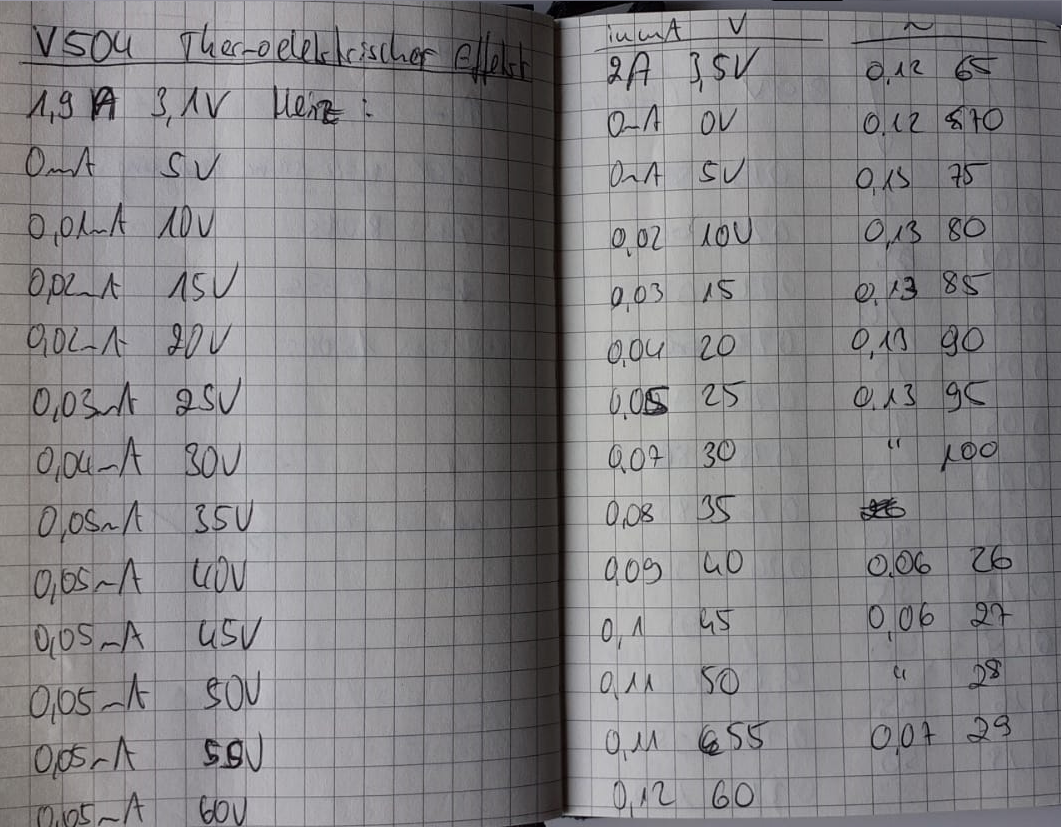
\includegraphics[width=8cm]{a1.png}
\caption{Originale Messdaten.}
\end{figure}
\begin{figure}[H]
\centering
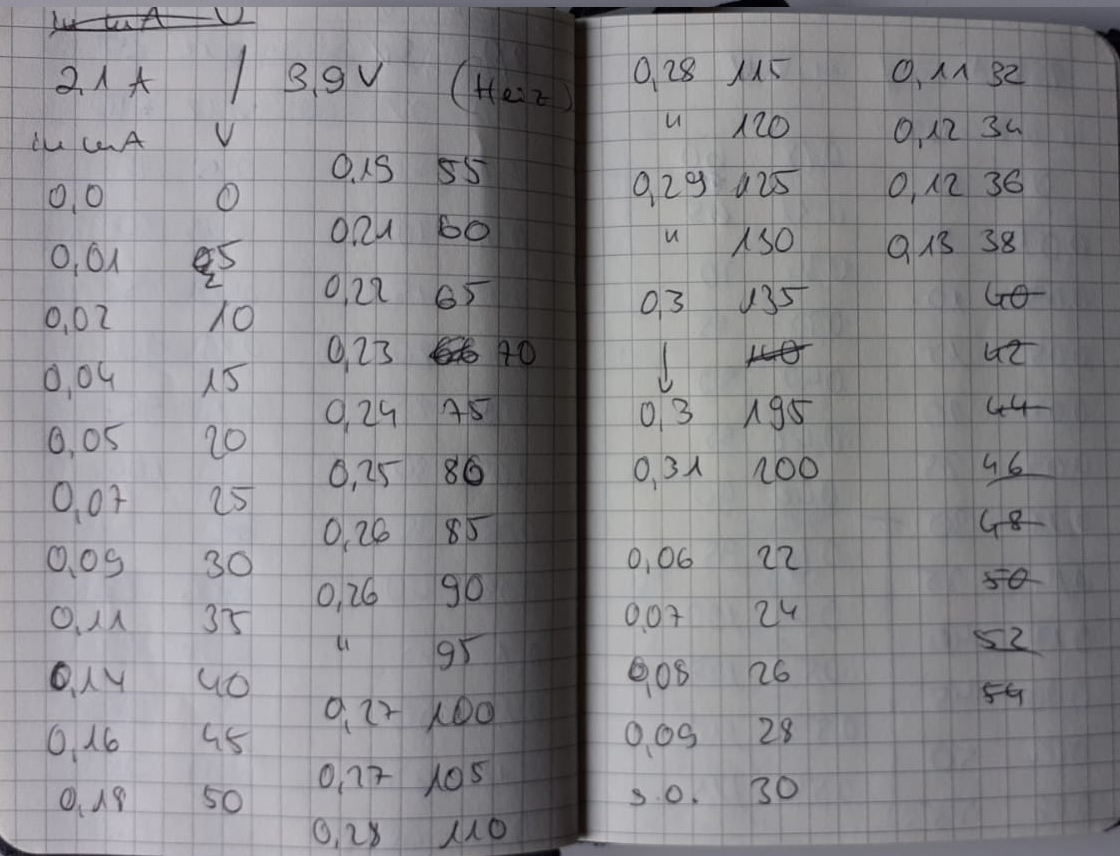
\includegraphics[width=8cm]{a2.png}
\caption{Originale Messdaten.}
\end{figure}
\begin{figure}[H]
\centering
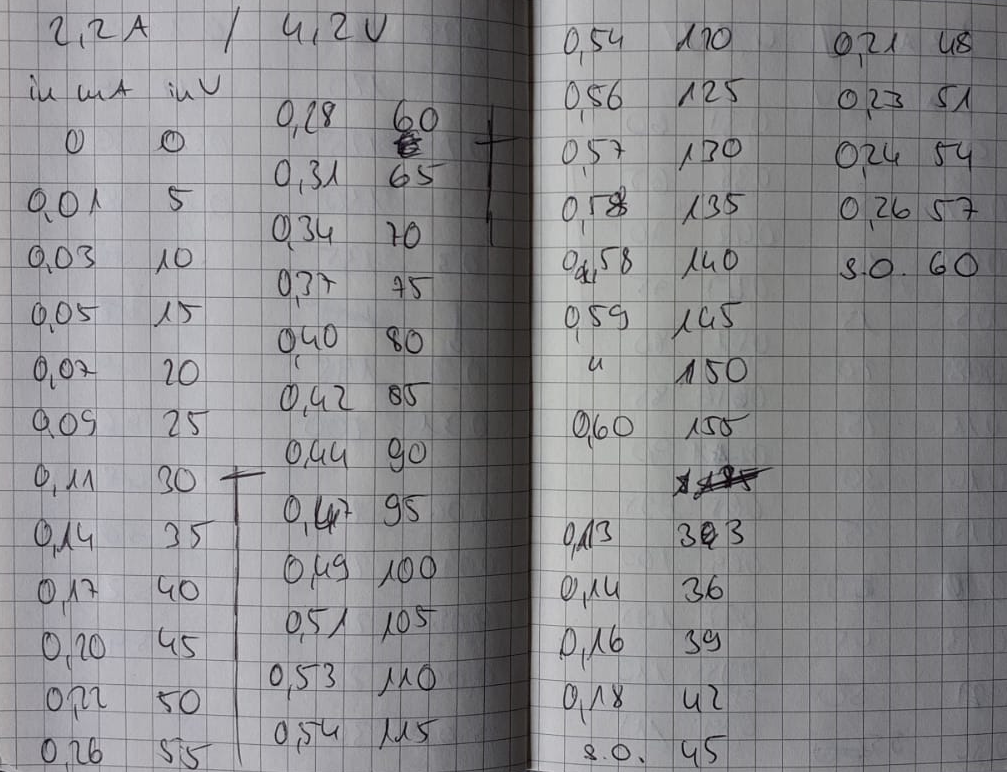
\includegraphics[width=8cm]{a3.png}
\caption{Originale Messdaten.}
\end{figure}
\begin{figure}[H]
\centering
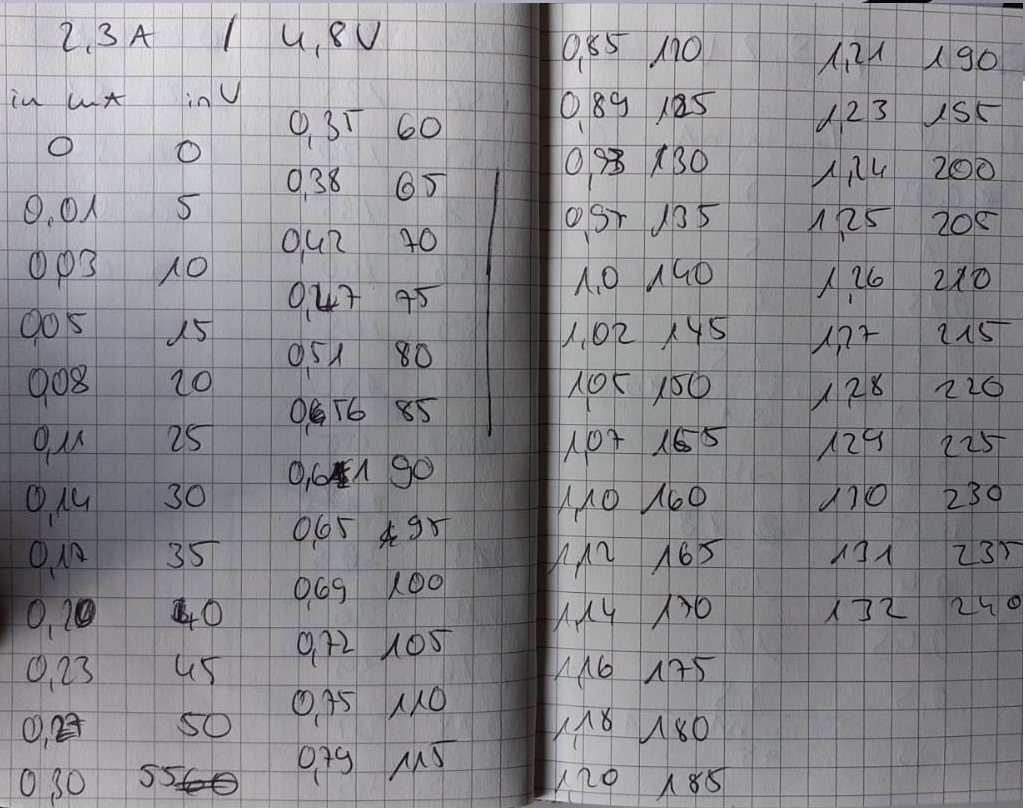
\includegraphics[width=8cm]{a4.png}
\caption{Originale Messdaten.}
\end{figure}
\begin{figure}[H]
\centering
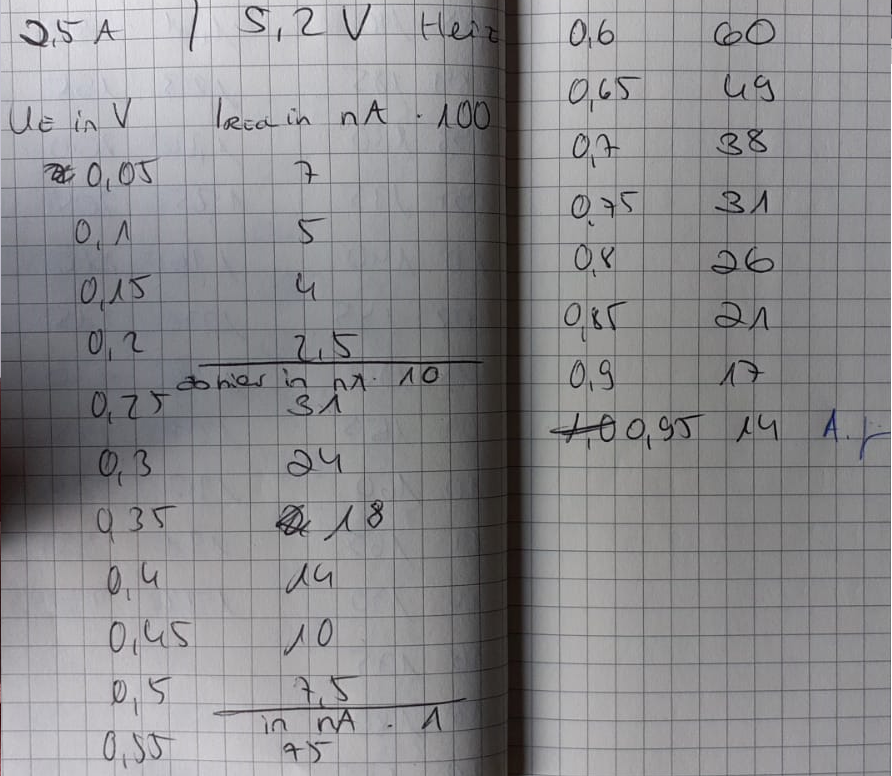
\includegraphics[width=8cm]{a5.png}
\caption{Originale Messdaten.}
\end{figure}
